\chapter{Zabezpečení dat proti chybám}
Při přenosu dat může dojít k jejich poškození. Abychom mohli ověřit korektnost přicházejících informací, tak je třeba zavézt bezpečnostní prostředky, které nám umožní odhalení chyb. Mezi tyto bezpečnostní prostředky patří i zabezpečovací kódy, kterými se budu v této kapitole zabývat.


\section{Exkluzivní disjunkce}
Někdy je možné se setkat i z pojmenováním exkluzivní součet, zkratkou XOR, případně značením $\oplus$. XOR je logická funkce, která se dá syntetizovat se základních logických funkcí AND či OR a NOT. Tato funkce často nalézá uplatnění v kryptografii, hlavně v hašovacích funkcích.

\begin{table}[!h]
  \caption{Tabulka hodnot logické funkce XOR, $A$ a $B$ jsou vstupy $Y$ je výstup}
  \begin{center}
  	\small
	  \begin{tabular}{|c|c||c|}
	    \hline
	    A & B & Y \\
	    \hline\hline
	    0 & 0 & 0 \\
	    \hline
	    0 & 1 & 1 \\
	    \hline
	    1 & 0 & 1 \\
	    \hline
	    1 & 1 & 0 \\
	    \hline
	  \end{tabular}
  \end{center}
\end{table}

\begin{itemize}
    \item Pokud $A = 0$, tak $Y = B$.
    \item Pokud $A = 1$, tak $Y = \overline{B}$, vznikne nám tedy negace.
    \item Výsledkem  $A \oplus B $ je logická jednička, pokud se její vstupy liší.
    \item XOR je funkce komutativní, takže nezáleží na pořadí dílčích kroků, to znamená, že $(A \oplus B) \oplus C = A \oplus (B \oplus C)$.
\end{itemize}

$$ Y = A \oplus B = \overline{A}B + A\overline{B} = (\overline{A} + \overline{B}) (A + B) $$




%Pokud detekujeme optickým přijímačem data, nikdy nemáme jistotu, že to jsou opravdu ta data, která vyslal náš vysílač a nebo jestli  nejsou poškozená. K tomu, abychom odhalili poškozená data, slouží zabezpečovací algoritmy. Fungují na tom principu, že kromě dat samotných se posílá ještě další redundantní informace spočítaná z přenášených dat. Některé zabezpečovací algoritmy jsou schopny kromě detekce chyb i chyby opravovat, například Hammingův kód, ale těmi se v této práci nehudu zabývat.

\section{Parita}
Parita je velmi jednoduchou cestou k zabezpečení dat. Ke každému slovu přenášených dat se přidá jeden redundantní bit označovaný jako paritní, jehož hodnota zrcadlí celkový počet jedniček. Paritu rozlišujeme na sudou a lichou. Nevýhodou parity je, že nedokáže odhalit několikanásobnou chybu.

\subsection{Sudá parita}
Paritní bit je nastaven tak, aby celkový počet jedniček v datovém slově včetně bitu paritního byl sudý. Můžeme ho spočítat jako exkluzivní součet všech bitů datového slova.
$$ P_{sudá} = b_0 \oplus b_1 \oplus ... \oplus b_n $$

\begin{figure}[H]
    \begin{center}
        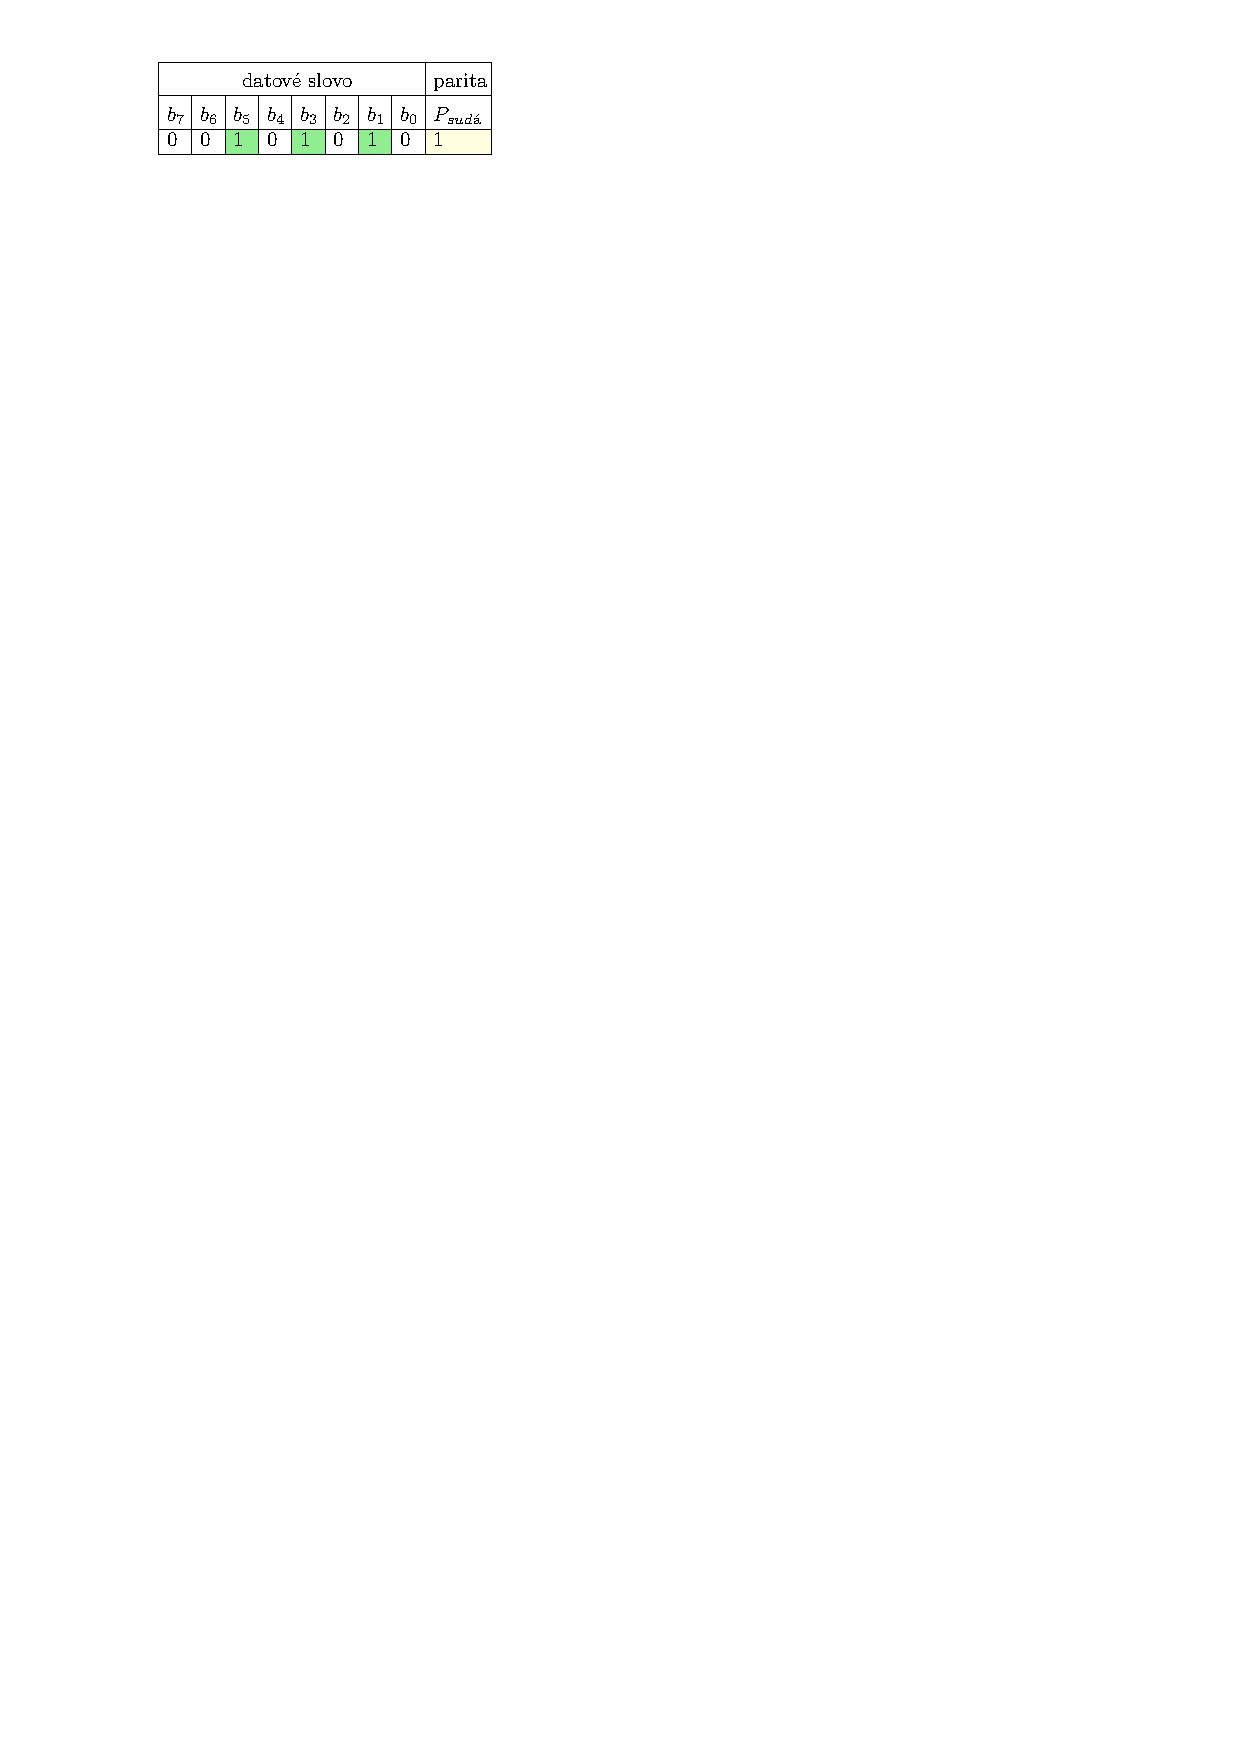
\includegraphics[scale=1]{img/parita_suda}
    \end{center}
    \caption{Ukázka sudé parity}
\end{figure}

\subsection{Lichá parita}
Paritní bit je nastaven tak, aby celkový počet jedniček v datovém slově včetně bitu paritního byl lichý. Můžeme ho spočítat obdobně jako sudý paritní bit, jen výsledek je třeba znegovat.
$$ P_{lichá} = \overline{ b_0 \oplus b_1 \oplus ... \oplus b_n } $$

\begin{figure}[H]
    \begin{center}
        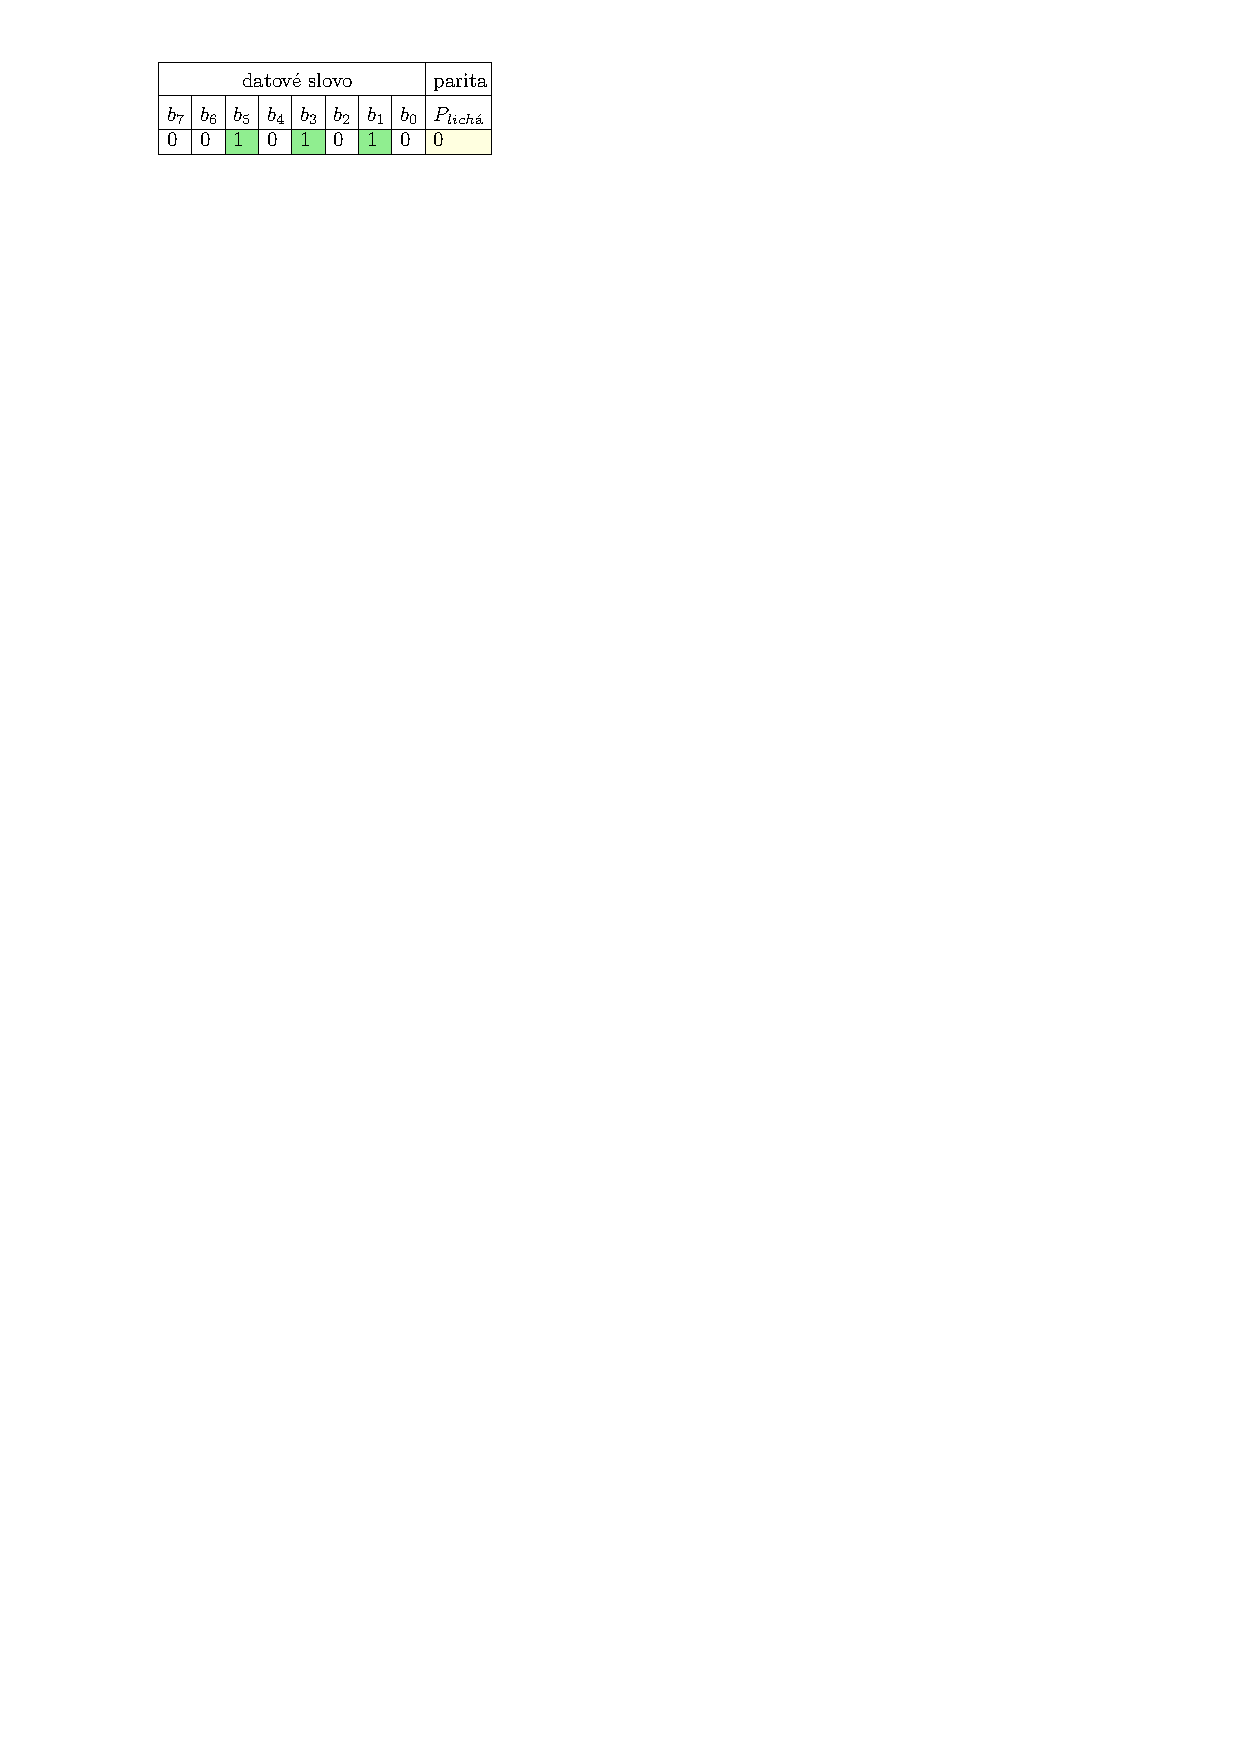
\includegraphics[scale=1]{img/parita_licha}
    \end{center}
    \caption{Ukázka liché parity}
\end{figure}

\section{Cyklický redundantní součet}
Používá se ke kontrole, zda-li máme nepoškozená data. Na konec přenášených dat se přidá několik redundantních bitů spočítaných pomocí speciální hašovací funkce \zkratka{CRC}. Po přijetí dat se může znovu spočítat \zkratka{CRC} pro přijatá data, které porovnáme z \zkratka{CRC}, které jsme přijali. Pokud budou kontrolní součty shodné, tak jsou i přijatá data v pořádku. Další možností je spočítat \zkratka{CRC} pro celá přijatá data včetně kontrolního součtu, pokud jsou přijatá data nepoškozená,  tak dostaneme bitový vektor plný nul.

Pravděpodobnost detekce chyby pomocí CRC, $n$ je délka generačního polynomu:
\begin{equation}
    P(n) = 1 - 2^{-n} \nonumber
\end{equation}

Čím více bitové \zkratka{CRC} pro kontrolu dat zvolíme, tím je větší pravděpodobnost odhalení chyby. Nejčastěji se používají \zkratka{CRC} o počtu bitů $8 \cdot 2^n$, kde $n \in \langle 0;~3\rangle$, ovšem je možné se ale setkat i s \zkratka{CRC} o jiných délkách, dokonce i s takovými, jejich binární logaritmus délky je necelé číslo.



\subsection{Generační polynom}
Generační polynom je bitový vektor, který by měl pokrývat nejčastější chyby, které se v našich datech objevují. Tento polynom je individuální pro každé přenosové nebo úložné médium. Vytvoření vhodného generačního polynomu je založené na shromažďování statistických údajů o přenášených datech. Na místech slova, kde je největší pravděpodobnost výskytu chyby se vloží jednička, tím je generační polynom vytvořen. Tento proces je ale velmi zdlouhavý a tak je jeho alternativou použít polynom již vytvořený jiným člověkem, několik polynomů pro různá přenosová média, jsou dostupné v \cite{crc-wiki}.

\subsection{Ukázka výpočtu kontrolního součtu}

Ukázka čtyřbitového \zkratka{CRC} pro znak *, který je reprezentován v ASCII kódování dekadickou hodnotou $(42)_{10}$, tedy $(00101010)_2$. S generačním polynomem $x^2+1$, který odpovídá bitovému vektoru $(101)_2$. Pro přehlednost udělám mezi jednotlivými nibbly mezeru a CRC oddělím velkou mezerou.

Data zprava doplníme čtyřmi nulami, tedy počtem nul, který odpovídá zvolené velikosti kontrolního součtu.
$$ (0010~1010~~~0000)_2 $$
Generační polynom přesuneme tak, aby jeho první jednička (zleva) byla na stejné pozici jako je první jednička dat (také zleva).
$$ (0010~1000~~~0000)_2 $$
Mezi daty a generačním polynomem provedeme exkluzivní součet.
\begin{eqnarray}
    (0010~1010~~~0000)_2  & \nonumber\\\underline{\oplus
    (0010~1000~~~0000)_2} & \nonumber\\
    (0000~0010~~~0000)_2  & \nonumber
\end{eqnarray}
Generační polynom posunujeme doprava, dokud se opět nepřekrývají jedničky a uděláme exkluzivní součet s předchozím výsledkem. Tento proces opakujeme, dokud na pozici dat nejsou samé nuly.
\begin{eqnarray}
    (0000~0010~~~0000)_2  & \nonumber\\\underline{\oplus
    (0000~0010~~~1000)_2} & \nonumber\\
    (0000~0000~~~1000)_2  & \nonumber
\end{eqnarray}
Vynulování jedniček na pozici dat dosáhneme hned při druhém opakování. Výsledkem kontrolního součtu je tedy bitový vektor $(1000)_2$.

Ten teď přidáme za data reprezentující znak *. Pro ověření správnosti spočítáme kontrolní součet, s tím rozdílem, že už nebudeme přidávat za data další čtyři nulové bity. Pokud nám vyjde aplikováním výše popsaného algoritmu nula, tak jsme postupovali správně.
\begin{eqnarray}
    (0010~1010~~~1000)_2  & \nonumber\\\underline{\oplus
    (0010~1000~~~0000)_2} & \nonumber\\
    (0000~0010~~~1000)_2  & \nonumber
\end{eqnarray}
\begin{eqnarray}
    (0000~0010~~~1000)_2  & \nonumber\\\underline{\oplus
    (0000~0010~~~1000)_2} & \nonumber\\
    (0000~0000~~~0000)_2  & \nonumber
\end{eqnarray}
Dvěma iteracemi algoritmu jsme dostali výsledek kýžený výsledek, takže data jsou v pořádku.

\subsection{Výpočet CRC pro obměnější data}
Při přenosu obměnějších dat (několik bytů) nastává problém, jakým způsobem pro ně efektivně počítat kontrolní součet. Využívám k tomu algoritmu, který jsem převzal z \cite{crc-wiki}.

\lstinputlisting{src/crc.cpp}

\begin{enumerate}
    \item Na začátku algoritmu přiřadíme do proměnné $crc$ vektor 32 jedniček.
    \item Poté každým bajtem dat modifikujeme hodnotu proměnné $crc$. Modifikace proměnné $crc$ spočívá v provedení exkluzivního součtu $crc$ s aktuálně zpracovávaným bytem dat a následného maskování výsledku pomocí bitového součinu s číslem 255. Touto operací vytvoříme číslo $\in \langle 0;~255 \rangle$, tedy 1~\jedn{B}.
    \item Pro takto upravený bajt je spočítán kontrolní součet.
    \item Provedeme exkluzivní součet mezi výsledkem 3. bodu a proměnnou $crc$ bitově posunutou o osm míst do prava.
    \item Výsledek 4. bodu uložíme do proměnné $crc$
    \item Opakujeme od 2. bodu dokud neprojdeme všechny datové bajty.
    \item Nakonec znegujeme hodnotu proměnné $crc$ ve které bude výsledek kontrolního součtu.
\end{enumerate}


Výpočet kontrolního součtu je možné zrychlit. Vzhledem k tomu, že probíhá nad známou množinou dat, tak si stačí před-počítat tabulku kontrolních součtů pro čísla $\in \langle 0; 256 \rangle$ a poté místo výpočtu jen přistupovat na daný řádek tabulky.
